\chapter{Espacios Métricos} 
{El análisis funcional es una rama abstracta de las matemáticas que se originó a partir del análisis clásico. Su desarrollo comenzó hace aproximadamente ochenta años, y en la actualidad los métodos y resultados del análisis funcional son importantes en diversos campos de las matemáticas y sus aplicaciones. El impulso provino del álgebra lineal, ecuaciones diferenciales ordinarias y parciales lineales, cálculo de variaciones, teoría de la aproximación y, en particular, de las ecuaciones integrales lineales, cuya teoría tuvo el mayor impacto en el desarrollo y promoción de las ideas modernas.

Los matemáticos observaron que los problemas de distintos campos a menudo comparten características y propiedades relacionadas. Este hecho se aprovechó para desarrollar un enfoque unificador y eficaz hacia tales problemas, unificación que se logra al omitir detalles no esenciales. Por lo tanto, la ventaja de un enfoque tan abstracto es que se concentra en los hechos esenciales, de modo que estos se hacen más evidentes, ya que la atención del investigador no se distrae con detalles sin importancia. En este sentido, el método abstracto es el más sencillo y económico para tratar sistemas matemáticos. Dado que cualquier sistema abstracto de este tipo tendrá, en general, diversas realizaciones concretas (modelos concretos), vemos que el método abstracto es bastante versátil en su aplicación a situaciones concretas. Ayuda a liberar el problema de su aislamiento y crea relaciones y transiciones entre campos que, en principio, no tienen contacto entre sí.

En el enfoque abstracto, generalmente se parte de un conjunto de elementos que satisfacen ciertos axiomas. La naturaleza de los elementos queda sin especificar, y esto se hace a propósito. La teoría, entonces, consiste en las consecuencias lógicas que se derivan de los axiomas y que se formulan como teoremas de una vez por todas. Esto significa que, de esta manera axiomática, se obtiene una estructura matemática cuya teoría se desarrolla de manera abstracta. Estos teoremas generales pueden aplicarse más tarde a varios conjuntos específicos que satisfacen dichos axiomas.

Por ejemplo, en álgebra se utiliza este enfoque en relación con cuerpos, anillos y grupos. En análisis funcional lo utilizamos en relación con espacios abstractos; estos son de fundamental importancia, y consideraremos algunos de ellos (espacios de Banach, espacios de Hilbert) con gran detalle. Veremos que en este contexto el concepto de ``espacio" se utiliza de manera muy amplia y sorprendentemente general. Un espacio abstracto será un conjunto de elementos (no especificados) que satisfacen ciertos axiomas. Y al elegir diferentes conjuntos de axiomas, obtendremos diferentes tipos de espacios abstractos.

La idea de utilizar espacios abstractos de manera sistemática se remonta a M. Fréchet (1906) y está justificada por su gran éxito. En este capítulo, consideramos los espacios métricos. Estos son fundamentales en el análisis funcional porque desempeñan un papel similar al de la recta real $\mathbf{R}$ en el cálculo. De hecho, generalizan a $\mathbf{R}$ y se han creado para proporcionar una base para el tratamiento unificado de problemas importantes en diversas ramas del análisis.

Primero definimos los espacios métricos y los conceptos relacionados, ilustrándolos con ejemplos típicos. Se discuten en detalle espacios especiales de importancia práctica.Se presta mucha atención al concepto de completitud, una propiedad que un espacio métrico puede o no tener. La completitud será un concepto clave a lo largo de todo el libro.


{\textbf{Conceptos importantes y orientación sobre el contenido principal}}


Un espacio métrico (véase 1.1-1) es un conjunto $X$ con una métrica definida en él. La métrica asocia a cada par de elementos (puntos) de $X$ una distancia. La métrica se define axiomáticamente, y los axiomas son sugeridos por ciertas propiedades simples de la distancia familiar entre puntos en la recta real $\mathbb{R}$ y el plano complejo $\mathbb{C}$. Ejemplos básicos (1.1-2 a 1.2-3) muestran que el concepto de un espacio métrico es notablemente general. Una propiedad adicional muy importante que puede tener un espacio métrico es la completitud (véase 1.4-3), la cual se discute en detalle en las secciones 1.5 y 1.6. Otro concepto de interés teórico y práctico es la separabilidad de un espacio métrico (véase 1.3-5). Los espacios métricos separables son más simples que los no separables.
}


\section{Espacio Métrico} 
{
En cálculo, estudiamos funciones definidas en la recta real $\mathbb{R}$. Una pequeña reflexión muestra que, en procesos de límites y muchas otras consideraciones, utilizamos el hecho de que en $\mathbb{R}$ tenemos disponible una función de distancia, llamada $d$, que asocia una distancia $d(x,y)=|x-y|$ con cada par de puntos
\(x, y \in \mathbb{R}\). La Figura 1 ilustra la notación. En el plano y en el espacio tridimensional ``ordinario", la situación es similar.
\begin{figure}[H]
    \centering
    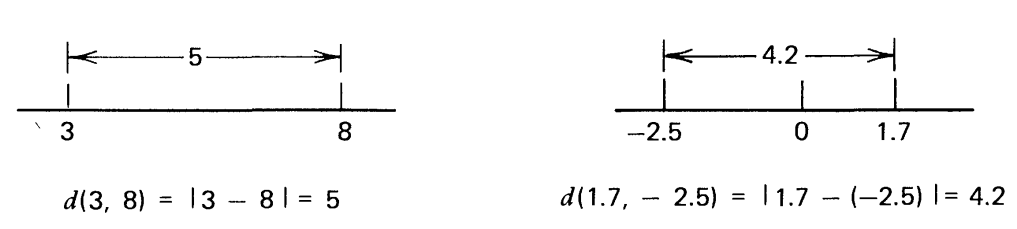
\includegraphics[width=0.5\textwidth]{img/metricSpace/1.png}
    \caption{Distancia en $\mathbb{R}$}
\end{figure}
En el análisis funcional, estudiaremos ``espacios''  y  ``funciones" más generales definidos sobre ellos. Llegamos a un concepto suficientemente general y flexible de "espacio" de la siguiente manera. Reemplazamos el conjunto de números reales subyacente en \(\mathbb{R}\) por un conjunto abstracto \(X\) (conjunto de elementos cuya naturaleza no se especifica) e introducimos sobre \(X\) una ``función de distancia'' que posee solo algunas de las propiedades más fundamentales de la función de distancia en \(\mathbb{R}\). Pero, ¿qué queremos decir con ``más fundamentales''?. 

Esta pregunta está lejos de ser trivial. De hecho, la elección y formulación de axiomas en una definición siempre requiere experiencia, familiaridad con problemas prácticos y una idea clara del objetivo a alcanzar. En el presente caso, un desarrollo de más de sesenta años ha conducido al siguiente concepto, que es fundamental y muy útil en el análisis funcional y sus aplicaciones.

\subsection{Definición}
Un espacio métrico es un par \((X, d)\), donde \(X\) es un conjunto y \(d\) es una métrica en \(X\) (o función de distancia en \(X\)), es decir, una función definida en \(X \times X\) tal que para todos \(x, y, z \in X\) tenemos:
\begin{align*}
    (M1)&\quad\quad d(x,y)>0,\quad\forall x\in X\\
    (M2)&\quad\quad d(x,y)=0 \leftrightarrow x=y\\
    (M3)&\quad\quad d(x,y)=d(y,x)\quad\quad &(Simetrico)\\
    (M4)&\quad\quad d(x,y)\leq d(x,z)+d(z,y)\quad\quad &(\text{Desigualdad Triangular})
\end{align*}
Algunos términos relacionados son los siguientes. \(X\) se llama normalmente el conjunto subyacente de \((X, d)\). Sus elementos se llaman puntos. Para \(x, y\) fijos, llamamos al número no negativo \(d(x, y)\) la distancia de \(x\) a \(y\). Las propiedades (M1) a (M4) son los axiomas de una métrica. 

El nombre ``desigualdad triangular'' está motivado por la geometría elemental, como se muestra en la Figura 1.2.

\begin{figure}[H]
    \centering
    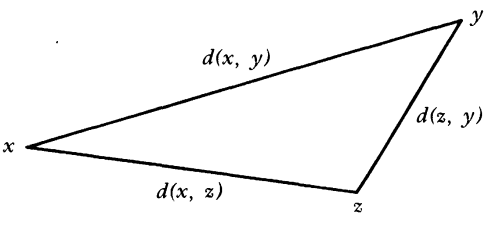
\includegraphics[width=0.4\textwidth]{img/metricSpace/2.png}
    \caption{Desiguldad Triangular en el plano}
\end{figure}
\newpage

A partir de (M4), obtenemos por inducción la desigualdad triangular generalizada. 
\begin{align}
    d(x_1,x_n)\leq d(x_1,x_2)+d(x_2,x_3)+\dots+d(x_{n-1},x_n)
\end{align}

En lugar de \((X, d)\), podemos simplemente escribir \(X\) si no hay peligro de confusión.

Un subespacio \((Y, \tilde{d})\) de \((X, d)\) se obtiene si tomamos un subconjunto \(Y \subseteq X\) y restringimos \(d\) a \(Y \times Y\); así, la métrica en \(Y\) es la restricción \(\tilde{d}\) que se llama la \textbf{métrica inducida} sobre \(Y\) por \(d\).
\[\tilde{d} = d|_{Y\times Y}\]

Ahora enumeraremos ejemplos de espacios métricos, algunos de los cuales ya son familiares para el lector. Para probar que estos son espacios métricos, debemos verificar en cada caso que se satisfacen los axiomas (M1) a (M4). 

Ordinariamente, para (M4) esto requiere más trabajo que para (M1) a (M3). Sin embargo, en nuestros ejemplos actuales esto no será difícil, por lo que podemos dejarlo al lector (cf. el conjunto de problemas). 
Espacios métricos más sofisticados para los cuales (M4) no se verifica tan fácilmente se incluyen en la próxima sección.

\subsection*{Ejemplos}

\subsection{Linea Real \texorpdfstring{$\mathbb{R}$}{R} }
Este es el conjunto de todos los números reales, tomado con la métrica usual definida por
\begin{align}
    d(x, y) = |x - y|
\end{align}
\subsection{Plano euclidiano \texorpdfstring{$\mathbb{R}^2$}{R} }
El espacio métrico \(\mathbb{R}^2\), llamado el plano euclidiano, se obtiene si tomamos el conjunto de pares ordenados de números reales, escritos como \(x = (x_1, x_2)\), \(y = (y_1, y_2)\), etc., y la métrica euclidiana definida por:
\begin{align}
    d(x,y)=\sqrt{(x_1-y_1)^2+(x_2-y_2)^2}
\end{align}

Otro espacio métrico se obtiene si elegimos el mismo conjunto que antes, pero con otra métrica \(d_1\) definida por:
\begin{align}
    d_1(x,y)=|x_1-y_1|+|x_2-y_2|
\end{align}
\begin{figure}[H]
    \centering
    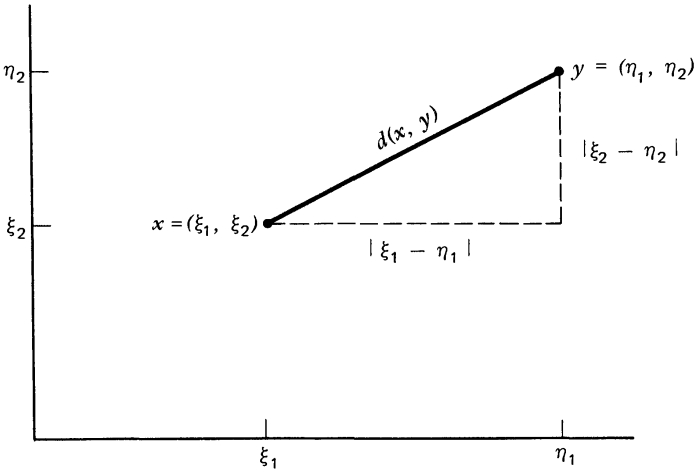
\includegraphics[width=0.5\textwidth]{img/metricSpace/3.png}
    \caption{Metrica Euclideana en el plano}
\end{figure}
Esto ilustra el hecho importante de que, a partir de un conjunto dado (que tenga más de un elemento), podemos obtener varios espacios métricos al elegir diferentes métricas. (El espacio métrico con la métrica \(d_1\) no tiene un nombre estándar. A veces se le llama \textbf{métrica del taxista}. ¿Por qué? \(\mathbb{R}^2\) a veces se denota como \(E^2\).)

\subsection{Espacio Euclidiano tridimensional \texorpdfstring{$\mathbb{R}^3$}{R} }
Este espacio métrico consiste en el conjunto de tripletas ordenadas de números reales \(x = (x_1, x_2, x_3)\), \(y = (y_1, y_2, y_3)\), etc., y la métrica Euclidiana definida por

}






\section{Ejemplos Adicionales de Espacios Métricos} 
\section{Conjunto Abierto, Conjunto Cerrado, Vecindad}
\section{Convergencia, Sucesión de Cauchy, Completitud}
\section{Ejemplos. Pruebas de Completitud}
\section{Compleción de Espacios Métricos} 